A key goal of our parallel design is to keep the threads as busy as possible and
to reduce inter-thread communication. Initially, the VM partitions the
application graph of $N$ nodes into $T$ subgraphs (the number of threads) and
then each thread will work on their own subgraph. During execution, threads can
steal nodes of other threads to keep themselves busy. The load balancing aspect
of the system is performed by our work scheduler that is based on a simple work
stealing algorithm.

Figure~\ref{fig:implementation:vm_overview} presents the layout of our virtual
machine for a program with six nodes and two running threads. Note that the
threads share the same memory space and communication between threads is
achieved using shared memory. Each thread space includes the nodes owned by the
thread (the dotted arrows represent the edges between nodes) and a \emph{Work
Queue}, which contains \textbf{active} nodes, i.e., nodes that have new facts to
process. This work queue is implemented as a linked list.  Initially, the work
queue is filled with all the nodes of the thread in order to derive the initial
facts. Not shown in the picture is the thread state flag, which represents the
state of thread and can be one of the following values:

\begin{itemize}

   \item \textbf{active}: The thread has a non-empty \emph{Work Queue} and/or is
      currently executing rules for a node.

   \item \textbf{idle}: The thread has no active nodes and is trying to
      synchronize with other threads to terminate the program.
   
   \item \textbf{stealing}: The thread is attemping to steal nodes from other
      threads.
\end{itemize}

Figure~\ref{fig:implementation:thread_states} presents the valid transitions for
the thread state flag.

\begin{figure}[ht]
   \centering
   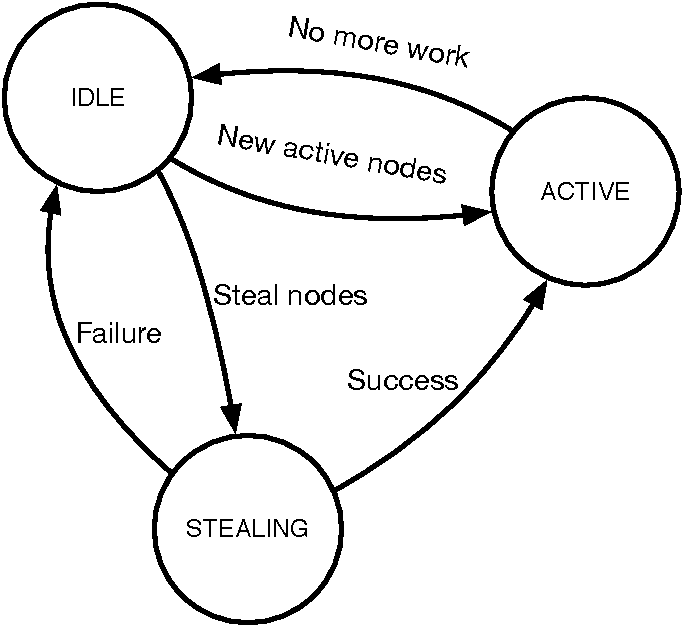
\includegraphics[width=0.4\textwidth]{figures/implementation/thread_states.pdf}
   \caption{The thread state machine as represented by the state flag. During
      the lifetime of a program, each thread goes through different states as
      specified by the state machine.}
   \label{fig:implementation:thread_states}
\end{figure}

The pseudo-code for the main thread loop is shown in
Fig.~\ref{alg:thread_work_loop}. In each round, a thread inspects its work queue
for active nodes, procedure \texttt{process\_node()} performs computation at the
node level.  When a thread's work queue is empty, it attempts to steal half of
the nodes from another thread. Starting from a random thread, it cycles through
all the threads to find one active thread. Eventually, there will be no more
work to do and the threads will go idle. There is a global atomic counter, a
global boolean flag and one state flag for each thread that are used to detect
termination. Once a thread goes idle, it decrements the global counter and
changes its flag to idle.  If the counter reaches zero, the global flag is set
to idle. Since every thread will be busy-waiting and checking the global flag,
they will detect the change and stop executing.

\begin{figure}
\begin{algorithm}[H]
   \KwData{Thread TH, THREADS}
   \While{true}{
      $node \longleftarrow TH.work\_queue.pop\_node()$ \;
      \uIf{$node$}{
         $TH.process\_node(node)$\;
      }
      \Else{
         \tcc{Need to steal some nodes.}
         $target \longleftarrow random(len(THREADS))$\;
         $i \longleftarrow 0$\;
         \For{$i < len(THREADS)$}{
            $target \longleftarrow (target + 1) \% len(THREADS)$\;
            $nodes = THREADS[target].steal\_half()$\;
            \If{$len(nodes) > 0$}{
               $TH.work\_queue.add\_to\_queue(nodes)$\;
               break\;
            }
            $i \longleftarrow i + 1$\;
         }
         \If{$len(TH.work\_queue) == 0$}{
            \tcc{try to terminate}
            $TH.become\_idle()$\;
            \If{$TH.synchronize\_termination()$}{
               \Return{}\;
            }
            \tcc{There's new nodes in the queue.}
            $TH.become\_active()$\;
         }
      }
 }
\end{algorithm}
\caption{Thread work loop: threads process active nodes from the work queue
   until no more active nodes are available. Node stealing using a \emph{steal
      half} strategy is employed when the thread has no more active nodes.}
 \label{alg:thread_work_loop}
\end{figure}

\begin{figure*}[t]
\centering
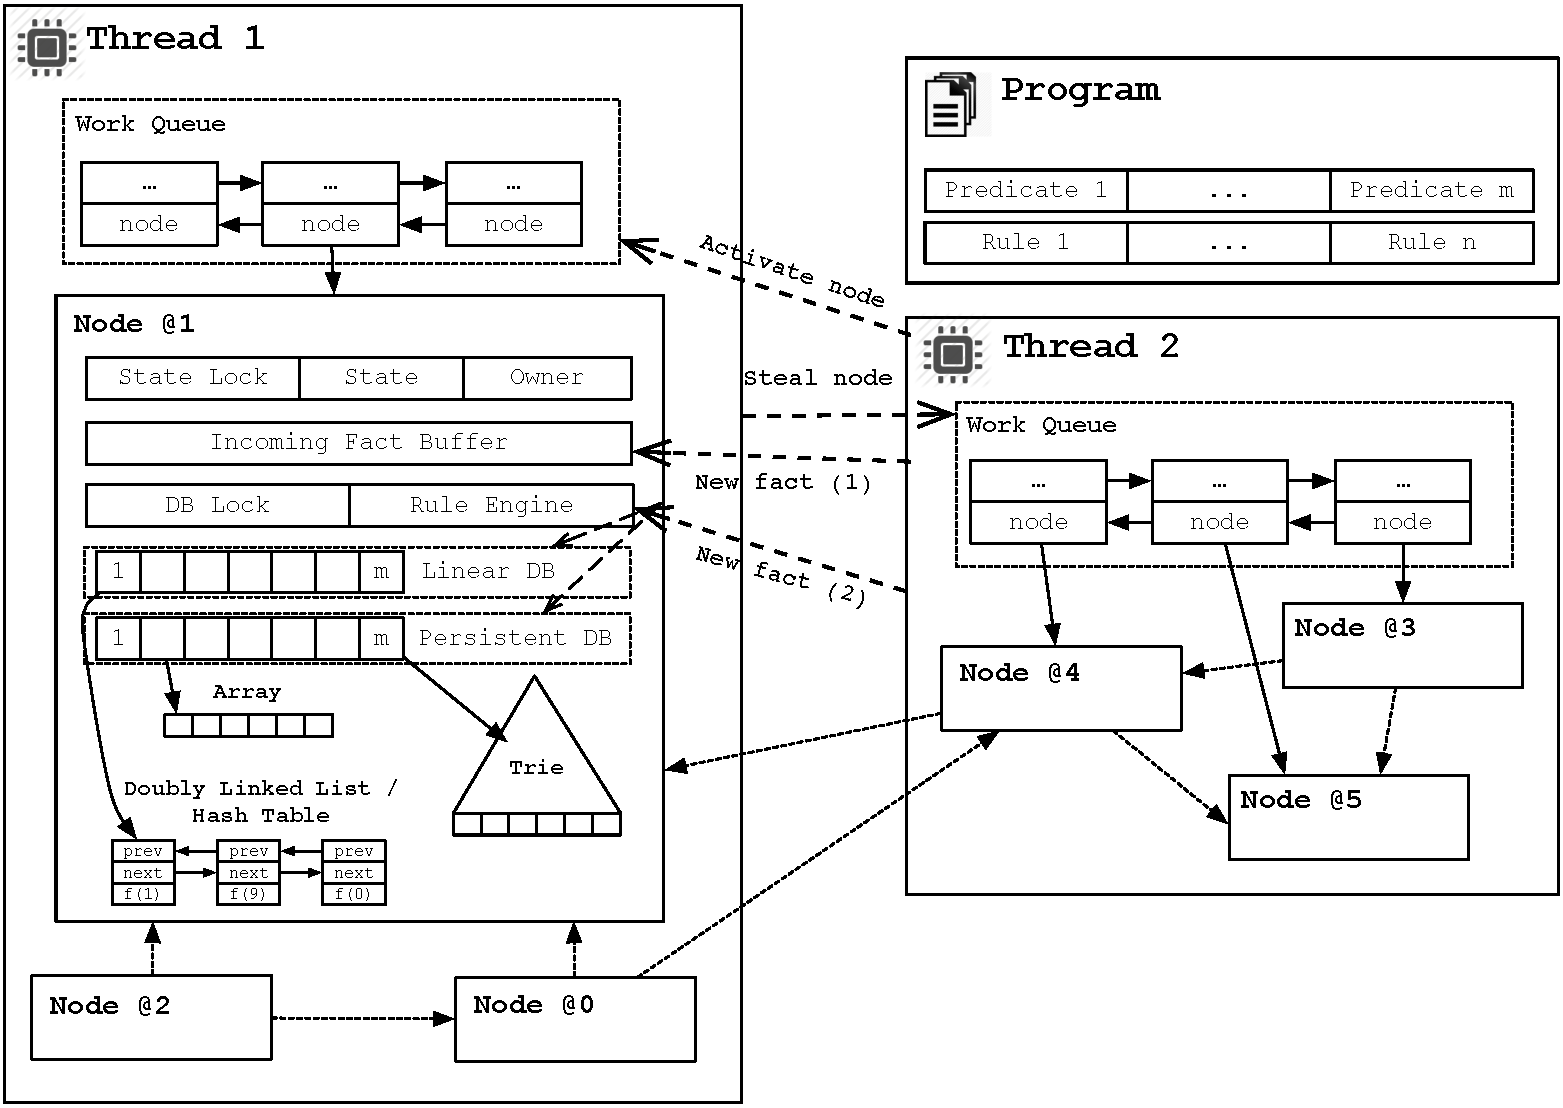
\includegraphics[width=\textwidth]{figures/implementation/vm_overview.pdf}
\caption{Layout of the virtual machine. Each thread has a work queue that
   contains active nodes (nodes with facts to process) that are processed one
   by one by the thread. Communication between threads happens when nodes
   send facts to nodes located in other threads.}
\label{fig:implementation:vm_overview}
\end{figure*}

Whenever a new fact is derived through rule derivation, we need to update the
data structures for the corresponding node. This is trivial if the thread that
derived the fact also owns the node. If that is not the case, then we have to
synchronize since multiple threads might be updating the same node's data
structures. For example, in Fig.~\ref{fig:implementation:vm_overview}, when
thread 2 derives a fact to node \texttt{@1} (owned by thread 1), it first locks
node \texttt{@1} using the \emph{Main Lock} and then it attempts to lock
\emph{DB Lock}, which gives thread 2 full access to the node. In this case,
thread 2 adds the new fact to the database (\emph{New fact (1)}) and to the rule
engine. However, if the \emph{DB Lock} could not be acquired because the node
\code{@1} is currently being executed, then the new fact is added to \emph{Fact
Buffer} (\emph{New fact (2)}). The facts stored in \emph{Fact Buffer} will then
be processed whenever the corresponding node's flag becomes active.

There is another thread interaction that might happen during fact derivation if
the node receiving a new fact is not active. In such case, the sending thread
needs to activate the node by pushing it to the \emph{Work Queue} of the target
thread. For example, consider again the situation in which thread 2 sends a new
fact to node \texttt{@1}. If node \texttt{@1} is not active, then thread 2 also
needs to activate \code{@1} by pushing it to the \emph{Work Queue} of thread 1.
After this synchronization point, the target thread is ensured to be active and
with a new node to process.

\subsection{Runtime Data Structures And Garbage Collection}

LM supports recursive types such as lists, arrays and structures. These compound
data structures are immutable and shared between multiple facts. Such structures
are stored in the heap of the VM and are managed through reference counting. For
instance, each list is a \emph{cons cell} with 3 fields: \texttt{tail}, the
pointer to the next element of the list; \texttt{head}, the element stored by
this element of the list; and \texttt{refs}, which counts the number of pointers
to this list element in the VM. The list is deleted from the heap whenever
\texttt{refs} is decremented to zero.

Nodes are also subject to garbage collection. If the database of a node becomes
empty and there are no references to the node from other logical facts, then the
node is deleted from the program. We keep around a small number of freed nodes
that can be reused immediately if another node is created.  We avoid garbage
collection schemes based on tracing since objects are created and discarded in
very specific points of the virtual machine and the runtime objects cannot
contain circular references. A reference counting mechanism is thus more
appropriate than a parallel tracing garbage collector which would entail pausing
the execution of the program to garbage collect all the unused objects.
